% Options for packages loaded elsewhere
% Options for packages loaded elsewhere
\PassOptionsToPackage{unicode}{hyperref}
\PassOptionsToPackage{hyphens}{url}
\PassOptionsToPackage{dvipsnames,svgnames,x11names}{xcolor}
%
\documentclass[
  spanish,
  10pt,
]{article}
\usepackage{xcolor}
\usepackage{amsmath,amssymb}
\setcounter{secnumdepth}{5}
\usepackage{iftex}
\ifPDFTeX
  \usepackage[T1]{fontenc}
  \usepackage[utf8]{inputenc}
  \usepackage{textcomp} % provide euro and other symbols
\else % if luatex or xetex
  \usepackage{unicode-math} % this also loads fontspec
  \defaultfontfeatures{Scale=MatchLowercase}
  \defaultfontfeatures[\rmfamily]{Ligatures=TeX,Scale=1}
\fi
\usepackage{lmodern}
\ifPDFTeX\else
  % xetex/luatex font selection
  \setmainfont[]{Arial}
\fi
% Use upquote if available, for straight quotes in verbatim environments
\IfFileExists{upquote.sty}{\usepackage{upquote}}{}
\IfFileExists{microtype.sty}{% use microtype if available
  \usepackage[]{microtype}
  \UseMicrotypeSet[protrusion]{basicmath} % disable protrusion for tt fonts
}{}
\makeatletter
\@ifundefined{KOMAClassName}{% if non-KOMA class
  \IfFileExists{parskip.sty}{%
    \usepackage{parskip}
  }{% else
    \setlength{\parindent}{0pt}
    \setlength{\parskip}{6pt plus 2pt minus 1pt}}
}{% if KOMA class
  \KOMAoptions{parskip=half}}
\makeatother
% Make \paragraph and \subparagraph free-standing
\makeatletter
\ifx\paragraph\undefined\else
  \let\oldparagraph\paragraph
  \renewcommand{\paragraph}{
    \@ifstar
      \xxxParagraphStar
      \xxxParagraphNoStar
  }
  \newcommand{\xxxParagraphStar}[1]{\oldparagraph*{#1}\mbox{}}
  \newcommand{\xxxParagraphNoStar}[1]{\oldparagraph{#1}\mbox{}}
\fi
\ifx\subparagraph\undefined\else
  \let\oldsubparagraph\subparagraph
  \renewcommand{\subparagraph}{
    \@ifstar
      \xxxSubParagraphStar
      \xxxSubParagraphNoStar
  }
  \newcommand{\xxxSubParagraphStar}[1]{\oldsubparagraph*{#1}\mbox{}}
  \newcommand{\xxxSubParagraphNoStar}[1]{\oldsubparagraph{#1}\mbox{}}
\fi
\makeatother


\usepackage{longtable,booktabs,array}
\usepackage{calc} % for calculating minipage widths
% Correct order of tables after \paragraph or \subparagraph
\usepackage{etoolbox}
\makeatletter
\patchcmd\longtable{\par}{\if@noskipsec\mbox{}\fi\par}{}{}
\makeatother
% Allow footnotes in longtable head/foot
\IfFileExists{footnotehyper.sty}{\usepackage{footnotehyper}}{\usepackage{footnote}}
\makesavenoteenv{longtable}
\usepackage{graphicx}
\makeatletter
\newsavebox\pandoc@box
\newcommand*\pandocbounded[1]{% scales image to fit in text height/width
  \sbox\pandoc@box{#1}%
  \Gscale@div\@tempa{\textheight}{\dimexpr\ht\pandoc@box+\dp\pandoc@box\relax}%
  \Gscale@div\@tempb{\linewidth}{\wd\pandoc@box}%
  \ifdim\@tempb\p@<\@tempa\p@\let\@tempa\@tempb\fi% select the smaller of both
  \ifdim\@tempa\p@<\p@\scalebox{\@tempa}{\usebox\pandoc@box}%
  \else\usebox{\pandoc@box}%
  \fi%
}
% Set default figure placement to htbp
\def\fps@figure{htbp}
\makeatother


% definitions for citeproc citations
\NewDocumentCommand\citeproctext{}{}
\NewDocumentCommand\citeproc{mm}{%
  \begingroup\def\citeproctext{#2}\cite{#1}\endgroup}
\makeatletter
 % allow citations to break across lines
 \let\@cite@ofmt\@firstofone
 % avoid brackets around text for \cite:
 \def\@biblabel#1{}
 \def\@cite#1#2{{#1\if@tempswa , #2\fi}}
\makeatother
\newlength{\cslhangindent}
\setlength{\cslhangindent}{1.5em}
\newlength{\csllabelwidth}
\setlength{\csllabelwidth}{3em}
\newenvironment{CSLReferences}[2] % #1 hanging-indent, #2 entry-spacing
 {\begin{list}{}{%
  \setlength{\itemindent}{0pt}
  \setlength{\leftmargin}{0pt}
  \setlength{\parsep}{0pt}
  % turn on hanging indent if param 1 is 1
  \ifodd #1
   \setlength{\leftmargin}{\cslhangindent}
   \setlength{\itemindent}{-1\cslhangindent}
  \fi
  % set entry spacing
  \setlength{\itemsep}{#2\baselineskip}}}
 {\end{list}}
\usepackage{calc}
\newcommand{\CSLBlock}[1]{\hfill\break\parbox[t]{\linewidth}{\strut\ignorespaces#1\strut}}
\newcommand{\CSLLeftMargin}[1]{\parbox[t]{\csllabelwidth}{\strut#1\strut}}
\newcommand{\CSLRightInline}[1]{\parbox[t]{\linewidth - \csllabelwidth}{\strut#1\strut}}
\newcommand{\CSLIndent}[1]{\hspace{\cslhangindent}#1}

\ifLuaTeX
\usepackage[bidi=basic]{babel}
\else
\usepackage[bidi=default]{babel}
\fi
\ifPDFTeX
\else
\babelfont{rm}[]{Arial}
\fi
% get rid of language-specific shorthands (see #6817):
\let\LanguageShortHands\languageshorthands
\def\languageshorthands#1{}


\setlength{\emergencystretch}{3em} % prevent overfull lines

\providecommand{\tightlist}{%
  \setlength{\itemsep}{0pt}\setlength{\parskip}{0pt}}



 


\usepackage{booktabs}
\usepackage{longtable}
\usepackage{array}
\usepackage{multirow}
\usepackage{wrapfig}
\usepackage{float}
\usepackage{colortbl}
\usepackage{pdflscape}
\usepackage{tabu}
\usepackage{threeparttable}
\usepackage{threeparttablex}
\usepackage[normalem]{ulem}
\usepackage{makecell}
\usepackage{xcolor}
% Paquetes necesarios
\usepackage{amsmath}
\usepackage{amssymb}
\usepackage{graphicx}
\usepackage{fancyhdr}
\usepackage{geometry}
\usepackage{booktabs}
\usepackage{dcolumn}
\usepackage{array}
\newcolumntype{d}[1]{D{.}{.}{#1}}
\usepackage{float}
\usepackage{adjustbox}
\renewcommand{\normalsize}{\fontsize{10pt}{12pt}\selectfont}

% Configuración de márgenes
\geometry{
  a4paper,
  left=1.5cm,
  right=1.5cm,
  top=1.5cm,
  bottom=2.5cm,
  includeheadfoot
}

% Configuración de encabezado y pie de página
\pagestyle{fancy}
\fancyhf{} % Limpia encabezado y pie de página

% Encabezado
\lhead{
\includegraphics[height=1.5cm]{logo.png}} % Logo en el encabezado
\chead{}
\rhead{\small Econometría: Prueba 1.}

% Ajuste de separación entre encabezado y contenido
\setlength{\headheight}{2cm} % Altura del encabezado
\setlength{\headsep}{1.5cm} % Distancia entre encabezado y contenido

% Pie de página
\lfoot{}
\cfoot{\thepage} % Número de página centrado
\rfoot{}
\makeatletter
\@ifpackageloaded{caption}{}{\usepackage{caption}}
\AtBeginDocument{%
\ifdefined\contentsname
  \renewcommand*\contentsname{Tabla de contenidos}
\else
  \newcommand\contentsname{Tabla de contenidos}
\fi
\ifdefined\listfigurename
  \renewcommand*\listfigurename{Listado de Figuras}
\else
  \newcommand\listfigurename{Listado de Figuras}
\fi
\ifdefined\listtablename
  \renewcommand*\listtablename{Listado de Tablas}
\else
  \newcommand\listtablename{Listado de Tablas}
\fi
\ifdefined\figurename
  \renewcommand*\figurename{Figura}
\else
  \newcommand\figurename{Figura}
\fi
\ifdefined\tablename
  \renewcommand*\tablename{Tabla}
\else
  \newcommand\tablename{Tabla}
\fi
}
\@ifpackageloaded{float}{}{\usepackage{float}}
\floatstyle{ruled}
\@ifundefined{c@chapter}{\newfloat{codelisting}{h}{lop}}{\newfloat{codelisting}{h}{lop}[chapter]}
\floatname{codelisting}{Listado}
\newcommand*\listoflistings{\listof{codelisting}{Listado de Listados}}
\makeatother
\makeatletter
\makeatother
\makeatletter
\@ifpackageloaded{caption}{}{\usepackage{caption}}
\@ifpackageloaded{subcaption}{}{\usepackage{subcaption}}
\makeatother
\usepackage{bookmark}
\IfFileExists{xurl.sty}{\usepackage{xurl}}{} % add URL line breaks if available
\urlstyle{same}
\hypersetup{
  pdfauthor={Amaru Simón Agüero Jiménez},
  pdflang={es},
  colorlinks=true,
  linkcolor={blue},
  filecolor={Maroon},
  citecolor={Blue},
  urlcolor={Blue},
  pdfcreator={LaTeX via pandoc}}


\title{\begin{center}
  
\includegraphics[height=4cm]{logo.png} \\[1cm]
  \Large Econometría \\
\end{center}}
\usepackage{etoolbox}
\makeatletter
\providecommand{\subtitle}[1]{% add subtitle to \maketitle
  \apptocmd{\@title}{\par {\large #1 \par}}{}{}
}
\makeatother
\subtitle{Prueba 1}
\author{Amaru Simón Agüero Jiménez}
\date{2025-05-13}
\begin{document}
\maketitle

\renewcommand*\contentsname{Tabla de contenidos}
{
\hypersetup{linkcolor=}
\setcounter{tocdepth}{3}
\tableofcontents
}

\section{Caso.}\label{caso.}

Simular un proceso generador de datos para el tiempo que le toma a una
persona, negociando sobre la venta de un artículo, llegar a un acuerdo.
Nos interesa conocer los mecanismos psicológicos que operan detrás de
las decisiones cooperativas de las personas frente a Conflictos de
interés (juegos de suma cero). Interpretaremos el tiempo como una medida
inversa de cooperación ---i.e., ante mayor disposición de las personas
para cooperar o compartir las ganancias de la negociación, menor debería
ser el tiempo necesario para llegar a un acuerdo.

Creemos que las personas que perciban mayores niveles de Conflicto de
intereses con su contraparte implementarán tácticas de negociación menos
conciliadoras y tardarán más tiempo en llegar a un acuerdo. Esperamos,
por lo tanto, una relación directa entre el Conflicto percibido y el
tiempo para alcanzar un acuerdo en la negociación. Esperamos, que esta
relación esté moderada por el rasgo de reciprocidad, donde personas con
perfiles de cooperación no-condicionales tenderían a cooperar
independientemente del Conflicto percibido.

Supondremos, para este ejercicio, que el tiempo necesario para ponerse
de acuerdo (\textbf{en segundos}) es determinado \textbf{exclusivamente}
por:

\begin{enumerate}
\def\labelenumi{\arabic{enumi}.}
\item
  La percepción de Conflicto de interés (\textbf{en puntaje \(z\)}), de
  los participantes en la ronda de negociación, que medimos con la
  escala psicométrica Situational Interdependence
  Scale\textsuperscript{1}.
\item
  El rasgo de reciprocidad (\textbf{dummy}), que medimos de la
  clasificación de los participantes como cooperadores
  condicionales/no-condicionales a partir de la técnica del Strategy
  Method (dCC)\textsuperscript{2}.
\item
  El rasgo de pro-socialidad (\textbf{en puntaje \(z\)}), que medimos de
  la escala Social Value Orientation (SVO)\textsuperscript{3}.
\end{enumerate}

La \textbf{variable independiente de interés} principal es la
\textbf{percepción de Conflicto de interés}.

\section{Proceso generador de datos.}\label{proceso-generador-de-datos.}

Simular un proceso de generación de datos según lo que se especifica a
continuación. Asumir que el tiempo, la percepción de Conflicto de
interés y la prosocialidad siguen distribuciones normales y que la
reciprocidad sigue una distribución de Bernoulli. Utilizar los
siguientes parámetros y semillas para generar los datos:

\begin{itemize}
\tightlist
\item
  muestra: \(n = 50\)
\item
  tiempo: \(\beta_0 = 350\), \(\beta_{Conflicto} = 20\),
  \(\beta_{Conflicto \times dCC} = 30\), \(\beta_{svo} = -25\)
\item
  error: \(\mathrm{E}(u) = 0\), \(\mathrm{Var}(u|x) = \sigma^2 = 80^2\),
  seed = 6
\item
  svo: \(\mu_{svo} = 0\), \(\sigma_{svo} = 1\), seed = 5
\item
  Conflicto: \(\mu_{Conflicto} = 0 - 0.5 \times svo\),
  \(\sigma_{Conflicto} = 1\), seed = 2
\item
  dcc: \(\mu_{dcc} = 0.7\), seed = 45
\end{itemize}

\newpage

\section{Pregunta 1.}\label{pregunta-1.}

Describir el comportamiento de las variables de la muestra.

\begin{enumerate}
\def\labelenumi{(\alph{enumi})}
\tightlist
\item
  Tomar estadísticas descriptivas de las variables. Incluir, al menos,
  la media, moda, mediana y el rango intercuartílico, cuando
  corresponda.
\end{enumerate}

\begin{table}[H]
\centering
\caption{\label{tab:unnamed-chunk-3}Estadísticas descriptivas de las variables}
\centering
\begin{tabular}[t]{lll}
\toprule
Variable & Estadístico & Valor\\
\midrule
 & Media & 358.92\\
\cmidrule{2-3}
 & Desviación Estándar & 108.71\\
\cmidrule{2-3}
 & Moda & 368.77\\
\cmidrule{2-3}
 & Mediana & 359.47\\
\cmidrule{2-3}
\multirow[t]{-5}{*}{\raggedright\arraybackslash Tiempo} & IQR & 150.41\\
\cmidrule{1-3}
 & Media & 0.04\\
\cmidrule{2-3}
 & Desviación Estándar & 1.15\\
\cmidrule{2-3}
 & Moda & -0.48\\
\cmidrule{2-3}
 & Mediana & 0.09\\
\cmidrule{2-3}
\multirow[t]{-5}{*}{\raggedright\arraybackslash Conflicto} & IQR & 1.81\\
\cmidrule{1-3}
 & Media & 0.06\\
\cmidrule{2-3}
 & Desviación Estándar & 1.07\\
\cmidrule{2-3}
 & Moda & -0.84\\
\cmidrule{2-3}
 & Mediana & -0.14\\
\cmidrule{2-3}
\multirow[t]{-5}{*}{\raggedright\arraybackslash SVO} & IQR & 1.66\\
\cmidrule{1-3}
 & Frecuencia de No Cooperador Condicional & 9 (18\%)\\
\cmidrule{2-3}
\multirow[t]{-2}{*}{\raggedright\arraybackslash DCC} & Frecuencia de Cooperador Condicional & 41 (82\%)\\
\bottomrule
\end{tabular}
\end{table}

\newpage

\begin{enumerate}
\def\labelenumi{(\alph{enumi})}
\setcounter{enumi}{1}
\tightlist
\item
  Tomar gráficos de densidad y boxplot para variables continuas y
  gráfico de barras para variable categórica.
\end{enumerate}

\begin{figure}

\centering{

\pandocbounded{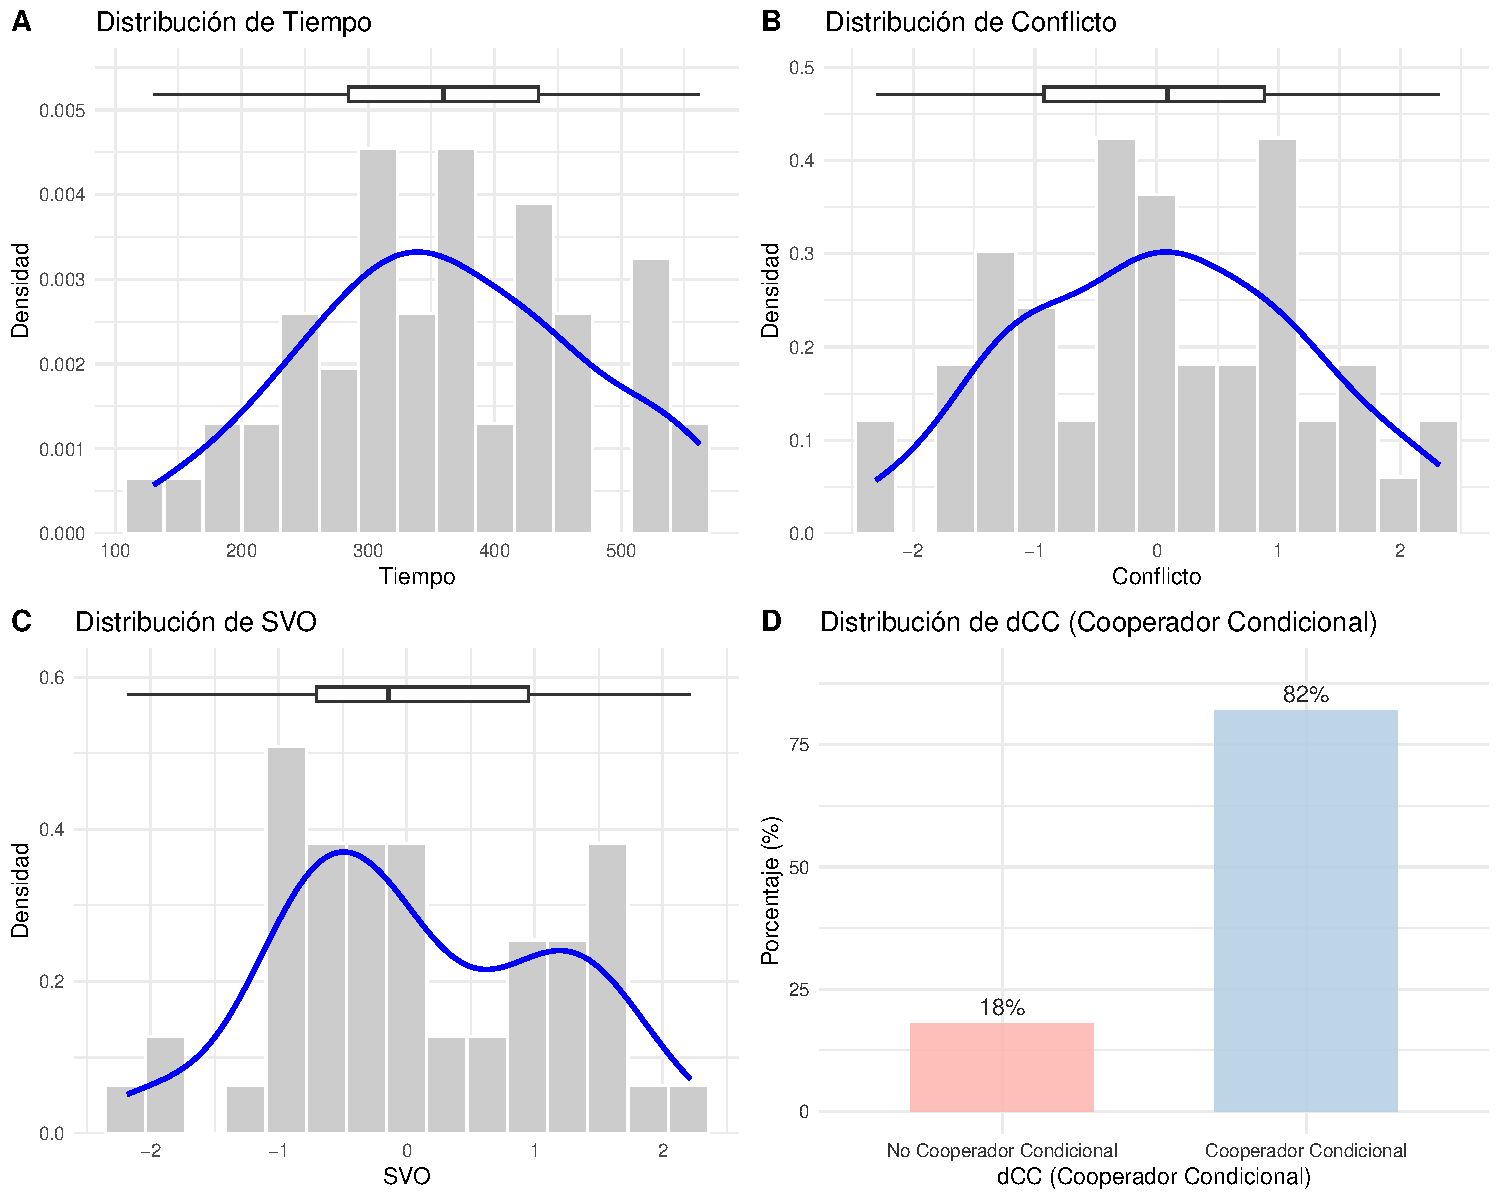
\includegraphics[keepaspectratio]{Prueba1_Amaru_Aguero_files/figure-pdf/fig-fig1-1.pdf}}

}

\caption{\label{fig-fig1}Distribución de las variables continuas y
categórica}

\end{figure}%

\begin{figure}

\centering{

\pandocbounded{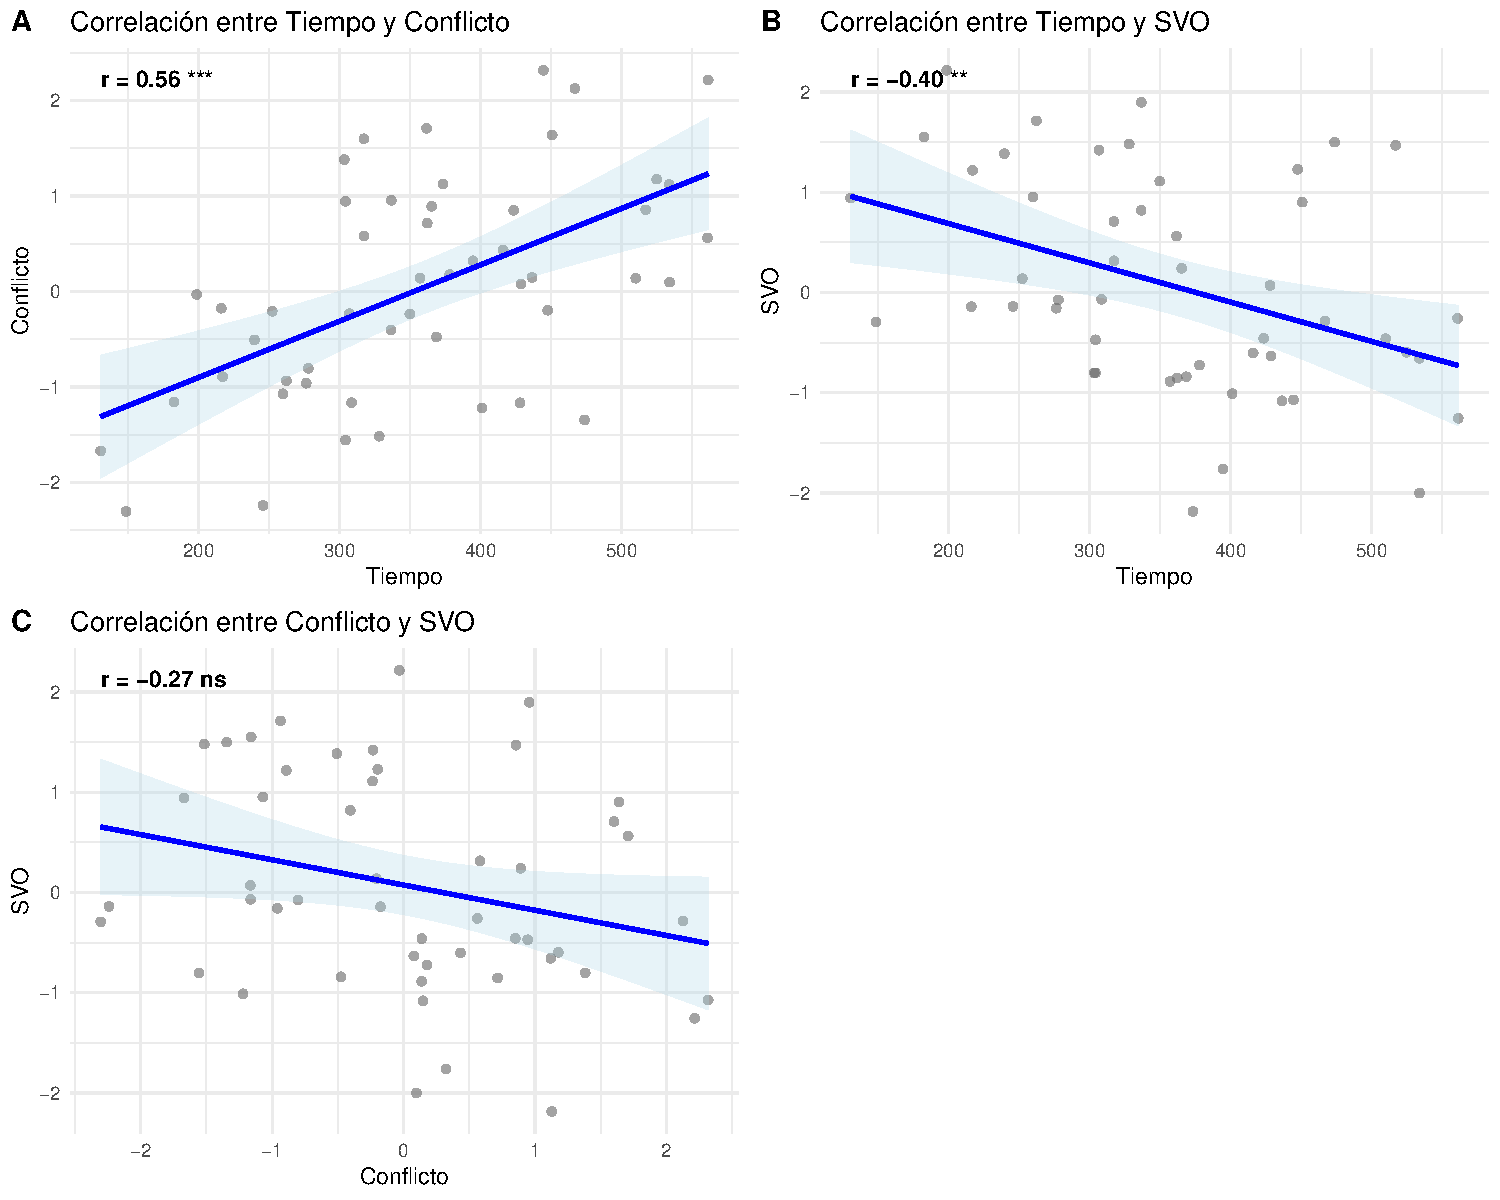
\includegraphics[keepaspectratio]{Prueba1_Amaru_Aguero_files/figure-pdf/fig-fig2-1.pdf}}

}

\caption{\label{fig-fig2}Correlación entre variables númericas}

\end{figure}%

\newpage

\section{Pregunta 2.}\label{pregunta-2.}

Ajustar los 6 Modelos lineales que se detallan a continuación, exportar
tabla con \texttt{stargazer()} e interpretar coeficientes y resultados
de cada Modelo. Comparar y explicar diferencias entre los Modelos.

\begin{enumerate}
\def\labelenumi{(\alph{enumi})}
\item
  \(tiempo \sim Conflicto\)
\item
  \(tiempo \sim Conflicto + svo\)
\item
  \(tiempo \sim Conflicto + dcc\)
\item
  \(tiempo \sim Conflicto + dcc + svo\)
\item
  \(tiempo \sim Conflicto + Conflicto \times dcc + dcc\)
\item
  \(tiempo \sim Conflicto + Conflicto \times dcc + dcc + svo\)
\end{enumerate}

En base a lo anterior se formulan los siguiente Modelos

\begin{itemize}
\item
  \(Modelo\;1:\; \text{tiempo}_i= \beta_0 + \beta_{\text{Conflicto}}\times\text{Conflicto}_i+ u_i\)
\item
  \(Modelo\;2:\; \text{tiempo}_i= \beta_0 + \beta_{\text{Conflicto}}\times\text{Conflicto}_i + \beta_{\text{SVO}}\times\text{SVO}_i+ u_i\)
\item
  \(Modelo \; 3:\; \text{tiempo}_i= \beta_0 + \beta_{\text{Conflicto}}\times\text{Conflicto}_i + \beta_{\text{dCC}}\times\text{dCC}_i+ u_i\)
\item
  \(Modelo\;4:\; \text{tiempo}_i = \beta_0 + \beta_{\text{Conflicto}}\times\text{Conflicto}_i+ \beta_{\text{SVO}}\times\text{SVO}_i+ \beta_{\text{dCC}}\times\text{dCC}_i+ u_i\)
\item
  \(Modelo\;5:\; \text{tiempo}_i= \beta_0 + \beta_{\text{Conflicto}}\times\text{Conflicto}_i + \beta_{\text{dCC}}\times\text{dCC}_i + \beta_{\text{Conflicto}\times\text{dCC}}\;      \times(\text{Conflicto}_i\times\text{dCC}_i) + u_i\)
\item
  \(Modelo\;6:\; \text{tiempo}_i = \beta_0 + \beta_{\text{Conflicto}}\times\text{Conflicto}_i + \beta_{\text{SVO}}\times\text{SVO}_i + \beta_{\text{dCC}}\times\text{dCC}_i + \beta_{\text{Conflicto}\times\text{dCC}}\times(\text{Conflicto}_i\times\text{dCC}_i) + u_i\)
\end{itemize}

\begin{table}[H] \centering 
  \caption{Resultados de los Modelos lineales ajustados} 
  \label{} 
\scriptsize 
\begin{tabular}{@{\extracolsep{5pt}}lcccccc} 
\\[-1.8ex]\hline 
\hline \\[-1.8ex] 
 & \multicolumn{6}{c}{\textit{Dependent variable:}} \\ 
\cline{2-7} 
\\[-1.8ex] & \multicolumn{6}{c}{Tiempo (segundos)} \\ 
 & Modelo 1 & Modelo 2 & Modelo 3 & Modelo 4 & Modelo 5 & Modelo 6 \\ 
\hline \\[-1.8ex] 
 Conflicto & 52.72$^{***}$ (11.32) & 45.90$^{***}$ (11.30) & 54.98$^{***}$ (11.36) & 48.16$^{***}$ (11.32) & 23.65 (29.91) & 15.42 (28.86) \\ 
  SVO &  & $-$27.13$^{*}$ (12.16) &  & $-$27.02$^{*}$ (12.05) &  & $-$27.35$^{*}$ (11.99) \\ 
  dCC Si &  &  & $-$44.60 (33.68) & $-$44.12 (32.32) & $-$34.93 (34.65) & $-$34.03 (33.17) \\ 
  Conflicto $\times$ dCC Si. &  &  &  &  & 36.57 (32.32) & 38.12 (30.94) \\ 
  Constant & 356.99$^{***}$ (12.90) & 359.00$^{***}$ (12.43) & 393.48$^{***}$ (30.38) & 395.09$^{***}$ (29.17) & 383.19$^{***}$ (31.62) & 384.38$^{***}$ (30.28) \\ 
 \hline \\[-1.8ex] 
Observations & 50 & 50 & 50 & 50 & 50 & 50 \\ 
R$^{2}$ & 0.31 & 0.38 & 0.34 & 0.40 & 0.35 & 0.42 \\ 
Adjusted R$^{2}$ & 0.30 & 0.35 & 0.31 & 0.36 & 0.31 & 0.37 \\ 
Residual Std. Error & 91.16 (df = 48) & 87.60 (df = 47) & 90.45 (df = 47) & 86.81 (df = 46) & 90.18 (df = 46) & 86.32 (df = 45) \\ 
F Statistic & 21.69$^{***}$ (df = 1; 48) & 14.23$^{***}$ (df = 2; 47) & 11.89$^{***}$ (df = 2; 47) & 10.28$^{***}$ (df = 3; 46) & 8.40$^{***}$ (df = 3; 46) & 8.18$^{***}$ (df = 4; 45) \\ 
\hline 
\hline \\[-1.8ex] 
\textit{Note:}  & \multicolumn{6}{r}{$^{*}$p$<$0.05; $^{**}$p$<$0.01; $^{***}$p$<$0.001} \\ 
\end{tabular} 
\end{table}

En la Tabla 2 se observan los resultados de los Modelos lineales con
método de estimación Ordinary Least Squares (OLS), bajo el contraste de
hipótesis en donde \(H_0:\beta_i=0\) y \(H_1:\beta_i\neq0\). Todos los
Modelos poseen un \(R^2\) estadisticamente distinto al Modelo nulo,
indicando un aumento de la capacidad predictiva al ingresar las
variables independientes.

En el \textbf{Modelo 1} el intercepto o \(\hat{\beta}_0\) es de 356.99
segundos y significativo (\emph{p}\textless0.001), representando el
tiempo promedio estimado cuando el Conflicto está en su valor medio (0
en escala \emph{z}). El coeficiente \(\hat{\beta}_{\text{Conflicto}}\)
es positivo (52.72) y significativo (\emph{p}\textless0.001), lo que
indica que existe un aumento de 52.72 segundos en el tiempo de
negociación por cada desviación estándar que aumenta la percepción de
Conflicto. De forma análoga, se espera una disminución de 52.72 segundos
si la percepción de Conflicto disminuye en una desviación estándar.
Respecto a los estadísticos \(R^2 = 0.31\) y
\(R^2_{\text{ajustado}} = 0.30\) muestran que el Conflicto por sí solo
explica aproximadamente 31 \% de la variabilidad del tiempo de
negociación, un aporte considerable para un único predictor.

En el \textbf{Modelo 2} el intercepto o \(\hat{\beta}_0\) es 359.00
segundos y significativo (\emph{p}\textless0.001), representando el
tiempo promedio estimado cuando el Conflicto y SVO están en su valor
medio (0 en escala \emph{z}). El coeficiente
\(\hat{\beta}_{\text{Conflicto}}\) se reduce a 45.90
(\emph{p}\textless0.001), manteniendo su efecto positivo. El coeficiente
de prosocialidad \(\hat{\beta}_{\text{SVO}}\) es --27.13 y significativo
(\emph{p}\textless0.05), lo que implica se acorta el tiempo de
negociación en 27.13 segundos por cada desviación estándar adicional en
SVO, reflejando que individuos más prosociales cooperan más rápido. El
ajuste mejora a \(R^2 = 0.38\) y \(R^2_{\text{ajustado}} = 0.35\),
indicando que SVO incrementa la varianza explicada en siete puntos
porcentuales respecto al \textbf{Modelo 1}.

Al comparar \(\hat{\beta}_{\text{Conflicto}}\) en ambos Modelos, con la
correlacion negativa observada en la Figura~\ref{fig-fig2} y dada la
siguiente relación en la Tabla 3.

\begin{longtable}[]{@{}
  >{\raggedright\arraybackslash}p{(\linewidth - 4\tabcolsep) * \real{0.2500}}
  >{\centering\arraybackslash}p{(\linewidth - 4\tabcolsep) * \real{0.3750}}
  >{\centering\arraybackslash}p{(\linewidth - 4\tabcolsep) * \real{0.3750}}@{}}
\caption{Dirección del sesgo en la estimación del coeficiente de SVO
según la correlación con la variable Conflicto}\tabularnewline
\toprule\noalign{}
\begin{minipage}[b]{\linewidth}\raggedright
\end{minipage} & \begin{minipage}[b]{\linewidth}\centering
\(\text{Corr}(x_{Conflicto}, x_{SVO}) > 0\)
\end{minipage} & \begin{minipage}[b]{\linewidth}\centering
\(\text{Corr}(x_{Conflicto}, x_{SVO}) < 0\)
\end{minipage} \\
\midrule\noalign{}
\endfirsthead
\toprule\noalign{}
\begin{minipage}[b]{\linewidth}\raggedright
\end{minipage} & \begin{minipage}[b]{\linewidth}\centering
\(\text{Corr}(x_{Conflicto}, x_{SVO}) > 0\)
\end{minipage} & \begin{minipage}[b]{\linewidth}\centering
\(\text{Corr}(x_{Conflicto}, x_{SVO}) < 0\)
\end{minipage} \\
\midrule\noalign{}
\endhead
\bottomrule\noalign{}
\endlastfoot
\(\hat\beta_{SVO} > 0\) & Positive bias & Negative bias \\
\(\hat\beta_{SVO} < 0\) & Negative bias & \textbf{Positive bias} \\
\end{longtable}

En el \textbf{Modelo 3} el intercepto, \(\hat{\beta}_0\) es de 393.48
segundos (\emph{p}\textless0.001), representa el tiempo promedio de
negociación estimado para un participante no condicional (dCC=0) cuando
la percepción de Conflicto se encuentra en su valor medio (0 en escala
\emph{z}). El \(\hat{\beta}_{\text{Conflicto}}\) aumenta en comparacion
al \textbf{Modelo 2} (dado el sesgo positivo por omitir SVO) y mantiene
su significancia estadistica (\emph{p}\textless0.001). Esto indica que
el tiempo de negociación se incrementa en 54.98 segundos , cuando la
percepción de Conflicto aumenta en una desviación estándar; de forma
análoga, disminuye en la misma magnitud si la percepción de Conflicto
cae una desviación estándar. En este Modelo tambien se observa una
reducción de 44.60 segundos cuando hay reciporcidad pero como el
\(\hat{\beta}_{dCC}\) es no signicativo (\emph{p}\textgreater0.05), este
coeficiente tiene una probabilidad que su valor sea 0 o incluso positivo
(dado su intervalo de confianza). Por último el Modelo explica un 34\%
de la variabilidad del tiempo (\(R^2 = 0.34\),
\(R^2_{\text{ajustado}} = 0.31\)), solo presenta una mejora modesta
respecto al \textbf{Modelo 1}.

En el \textbf{Modelo 4} el intercepto \(\hat{\beta}_0\) es de 395.09
segundos (\emph{p}\textless0.001) e indica el tiempo esperado para un
participante no condicional (dCC = 0), con valores medios de Conflicto y
SVO (0 en escala \emph{z}). El coeficiente
\(\hat{\beta}_{\text{Conflicto}}\) se reduce nuevamente a 48.16
(\emph{p}\textless0.001) (Por sesgo positivo de SVO sobre Conflicto).
Esto indica el tiempo aumenta en 48.16 segundos por Un aumento de una
desviación estándar en Conflicto. Por otra parte, el coeficiente de
prosocialidad \(\hat{\beta}_{\text{SVO}}\) es --27.02 y significativo
(\emph{p}\textless0.05), reduciendo el tiempo de negociación en 27.02
segundos por cada desviación estándar adicional en orientación prosocial
(SVO). Esto nuevamente refleja que los individuos más prosociales
cooperan con mayor rapidez. El coeficiente asociado a la reciprocidad
\(\hat{\beta}_{dCC}\) sigue siendo negativo (--44.12 segundos) pero no
significativo. Con \(R^2 = 0.40\) y \(R^2_{\text{ajustado}} = 0.36\),
este Modelo incrementa la varianza explicada hasta el 40\%, subrayando
la importancia conjunta del Conflicto y la prosocialidad.

En el \textbf{Modelo 5} se incorpora la interacción Conflicto × dCC. El
intercepto, \(\hat{\beta}_0 = 383.19\) segundos
(\emph{p}\textless0.001), corresponde al tiempo promedio para un
participante no condicional cuando la percepción de Conflicto tiene
promedio 0 (0 en escala \emph{z}). El ingreso de la interación provoca
la perdida de la significancia del coeficiente
\(\hat{\beta}_{\text{Conflicto}}\), mantiene la no significancia del
coeficiente \(\hat{\beta}_{dCC}\) y la interación con el coeficiente
\(\hat{\beta}_{Conflicto \times dCC}\) tambien es no significativa.
Respecto al ajuste global (\(R^2 = 0.35\),
\(R^2_{\text{ajustado}} = 0.31\)) permanece por debajo del obtenido
cuando se incluye SVO (\textbf{Modelo 4}).

En el \textbf{Modelo 6}, que combina Conflicto, SVO, dCC y su
interacción, el intercepto se estima en \(\hat{\beta}_0 = 384.38\)
segundos (\emph{p}\textless0.001)e indica el tiempo esperado para un
participante no condicional con valores medios de Conflicto y SVO (0 en
escala \emph{z}) y dCC: No.~Entre los participantes no condicionales, el
Conflicto muestra un coeficiente de 15.42 segundos por desviación
estándar, sin significancia estadística. La orientación prosocial
mantiene un efecto negativo robusto: El tiempo de negociación se reduce
en 27.35 segundos (\emph{p} \textless0.05) por cada desviación estándar
extra en SVO. Ni el coeficiente principal de reciprocidad
\(\hat\beta_{dCC}\) (--34.03 segundos) ni el coeficiente de interacción
\(\hat{\beta}_{Conflicto \times dCC}\) (38.12 segundos) resultan
significativos. Pese a ello, el Modelo muestra el mayor ajuste global,
explicando el 42 \% de la variación observada (\(R^2 = 0.42\),
\(R^2_{\text{ajustado}} = 0.37\)); la ganancia respecto al
\textbf{Modelo 4} es modesta y se atribuye principalmente a la mayor
flexibilidad del Modelo más que a evidencia estadística de un efecto de
moderación.

En conjunto, estos resultados reafirman el tiempo de negociación se
incrementa con un aumento en la percepción de Conflicto y que la
orientación prosocial lo reduce, mientras que los efectos vinculados a
la reciprocidad y su interacción con el Conflicto no son significativos
con la muestra actual.

\section{Pregunta 3.}\label{pregunta-3.}

¿Cuál Modelo cree que especifica correctamente la hipótesis a probar y
por qué?

La hipótesis planteada sostiene que \textbf{el tiempo de negociación es
infleunciado por la percepción de Conflicto} y que este \textbf{efecto
se ve moderado por el tipo de cooperador} (dCC: cooperador condicional =
0, cooperador incondicional = 1).

Formalmente: \(H_0:\;\beta_{\text{Conflicto}\times\text{dCC}} = 0\)
frente a \(H_1:\;\beta_{\text{Conflicto}\times\text{dCC}} \neq 0\).

Para operacionalizarla, el Modelo que incluye todos los términos
necesarios es el \textbf{Modelo 6}:
\(\text{tiempo}_i = \beta_0 + \beta_{\text{Conflicto}}\times\text{Conflicto}_i + \beta_{\text{SVO}}\times\text{SVO}_i + \beta_{\text{dCC}}\times\text{dCC}_i + \beta_{\text{Conflicto}\times\text{dCC}}\times(\text{Conflicto}_i\times\text{dCC}_i) + u_i\)
Al estimar el \textbf{Modelo 6} ninguno de los coeficientes asociados a
la moderación de conflcito es estadísticamente significativo
(\emph{p}\textgreater0,05). Esta pérdida de significancia en comapracion
a los \textbf{Modelos 1 , 2, 3 y 4} se explica, en gran medida, por dos
factores: la multicolinealidad inducida entre \emph{Conflicto} y el
término de interacción, que eleva los errores estándar de
\(\beta_{\text{Conflicto}}\) y
\(\beta_{\text{Conflicto}\times\text{dCC}}\), y el tamaño muestral
reducido (n = 50), que limita la potencia para detectar efectos
moderadores de magnitud moderada.

Aunque \textbf{Modelo 6} captura fielmente la hipótesis teórica, su leve
ganancia de ajuste (\(\Delta R^2 = 0,01\)) no compensa la mayor
complejidad ni el aumento en la varianza de los estimadores. Por el
contrario, el Modelo \textbf{Modelo 4}:
\(\text{tiempo}_i = \beta_0 + \beta_{\text{Conflicto}}\times\text{Conflicto}_i+ \beta_{\text{SVO}}\times\text{SVO}_i+ \beta_{\text{dCC}}\times\text{dCC}_i+ u_i\)
presenta coeficientes \(\beta_{\text{Conflicto}}\),
\(\beta_{\text{SVO}}\) y \(\beta_{\text{dCC}}\) significativos, evita la
colinealidad excesiva, evita el sesgo positivio de variable omitida de
SVO y conserva la parsimonia, ofreciendo una interpretación más estable
y directa del efecto principal de Conflicto controlando por SVO y dCC.

\section{Pregunta 4.}\label{pregunta-4.}

Repetir punto 2 volviendo a tomar una muestra de tiempo con
\(\beta_{Conflicto \times dCC} = 10\).

\begin{table}[H] \centering 
  \caption{Resultados de los Modelos lineales ajustados $\beta_{Conflicto \times dcc}$ = 10} 
  \label{} 
\scriptsize 
\begin{tabular}{@{\extracolsep{5pt}}lcccccc} 
\\[-1.8ex]\hline 
\hline \\[-1.8ex] 
 & \multicolumn{6}{c}{\textit{Dependent variable:}} \\ 
\cline{2-7} 
\\[-1.8ex] & \multicolumn{6}{c}{Tiempo (segundos)} \\ 
 & Modelo 1.2 & Modelo 2.2 & Modelo 3.2 & Modelo 4.2 & Modelo 5.2 & Modelo 6.2 \\ 
\hline \\[-1.8ex] 
 Conflicto & 35.86$^{**}$ (11.16) & 29.00$^{*}$ (11.11) & 37.85$^{**}$ (11.24) & 30.99$^{**}$ (11.18) & 23.65 (29.91) & 15.42 (28.86) \\ 
  SVO &  & $-$27.29$^{*}$ (11.96) &  & $-$27.19$^{*}$ (11.90) &  & $-$27.35$^{*}$ (11.99) \\ 
  dCC Si &  &  & $-$39.31 (33.31) & $-$38.83 (31.91) & $-$34.93 (34.65) & $-$34.03 (33.17) \\ 
  Conflicto $\times$ dCC Si. &  &  &  &  & 16.57 (32.32) & 18.12 (30.94) \\ 
  Constant & 355.69$^{***}$ (12.71) & 357.71$^{***}$ (12.22) & 387.85$^{***}$ (30.05) & 389.47$^{***}$ (28.80) & 383.19$^{***}$ (31.62) & 384.38$^{***}$ (30.28) \\ 
 \hline \\[-1.8ex] 
Observations & 50 & 50 & 50 & 50 & 50 & 50 \\ 
R$^{2}$ & 0.18 & 0.26 & 0.20 & 0.28 & 0.21 & 0.29 \\ 
Adjusted R$^{2}$ & 0.16 & 0.23 & 0.17 & 0.24 & 0.15 & 0.22 \\ 
Residual Std. Error & 89.84 (df = 48) & 86.14 (df = 47) & 89.47 (df = 47) & 85.71 (df = 46) & 90.18 (df = 46) & 86.32 (df = 45) \\ 
F Statistic & 10.33$^{**}$ (df = 1; 48) & 8.22$^{***}$ (df = 2; 47) & 5.90$^{**}$ (df = 2; 47) & 6.03$^{**}$ (df = 3; 46) & 3.96$^{*}$ (df = 3; 46) & 4.54$^{**}$ (df = 4; 45) \\ 
\hline 
\hline \\[-1.8ex] 
\textit{Note:}  & \multicolumn{6}{r}{$^{*}$p$<$0.05; $^{**}$p$<$0.01; $^{***}$p$<$0.001} \\ 
\end{tabular} 
\end{table}

En la Tabla 4 se observa los resutados de los Modelos lineales ajustados
con el nuevo valor de \(\beta_{Conflicto \times dCC}\) = 10. Todos los
Modelos poseen un \(R^2\) estadisticamente distinto al Modelo nulo,
indicando un aumento de la capacidad predictiva al ingresar las
variables independientes, pero hay Modelos con coeficientes menos
significativos como el \textbf{Modelo 5.2}.

Ahora en particular para el \textbf{Modelo 1.2}, se observa que tanto el
intercepto (\(\hat{\beta}_{0}\) = 355.69) como el coeficiente para
Conflicto (\(\hat{\beta}_{Conflicto}\)) son significativos. Este Modelo,
con un \(R^2 = 0.18\) y \(R^2_{ajustado} = 0.16\), menor que el
\textbf{Modelo 1} con un \(\beta_{Conflicto \times dCC}\) = 30,
(disminución del efecto de la interacción). Este Modelo tambien indica
que hay un aumento de tiempo de negociación por un aumento en una
desvision estadar de la percepción de Conflicto.

En el \textbf{Modelo 2.2}, los coeficientes para el intercepto
(\(\hat{\beta}_{0}\) = 357.71), Conflicto (\(\hat{\beta}_{Conflicto}\) =
29.00\^{}) y SVO (\(\hat{\beta}_{SVO}\) = -27.29) son todos
significativos. El Modelo presenta un \(R^2 = 0.26\) y un
\(R^2_{ajustado} = 0.23\), tambien menor que el \textbf{Modelo 2} .
Estos resultados sugieren que mientras el Conflicto incrementa el tiempo
de negociación, una mayor orientación al valor social (SVO o
prosocialidad) lo disminuye de forma significativa, mejorando el ajuste
general en comparación con el \textbf{Modelo 1.2}.

El \textbf{Modelo 3.2} muestra coeficientes significativos para el
intercepto (\(\hat{\beta}_{0}\) = 387.85) y para Conflicto
(\(\hat{\beta}_{Conflicto}\) = 37.85\^{}). Sin embargo, el coeficiente
para la variable dCC (ser cooperador condicional, \(\hat{\beta}_{dCC}\)
= -38.83) no resulta estadísticamente significativo. El Modelo tiene un
\(R^2 = 0.20\) y un \(R^2_{ajustado}\) = 0.17, indicando que el tipo de
cooperador dCC no tiene un impacto discernible en el tiempo de
negociación en este Modelo.

Respecto al \textbf{Modelo 4.2}, este presenta coeficientes
significativos para el intercepto (\(\hat{\beta}_{0}\) = 389.47),
Conflicto (\(\hat{\beta}_{Conflicto}\) = 30.99) y SVO
(\(\hat{\beta}_{SVO}\) = -27.19). Al igual que en el Modelo anterior, el
coeficiente para dCC Si (\(\hat{\beta}_{dCC}\) = -39.31) no es
significativo. Con un \(R^2 = 0.28\) y un \(R^2_{ajustado} = 0.24\),
este Modelo ofrece un buen balance, mostrando que el Conflicto aumenta
el tiempo y SVO lo disminuye, sin un efecto claro de dCC.

Para el \textbf{Modelo 5.2}, únicamente el intercepto
(\(\hat{\beta}_{0}\) = 383.19) es significativo. Los coeficientes para
Conflicto (\(\hat{\beta}_{Conflicto}\) = 23.65), dCC Si
(\(\hat{\beta}_{dCC}\) = -34.93) y la interacción Conflicto x dCC Si
(\(\hat{\beta}_{Conflicto \times dCC}\) = 16.57) no son estadísticamente
significativos. El \(R^2 = 0.21\) y el \(R^2_{ajustado} = 0.15\)
sugieren que la inclusión de la interacción, en estas condiciones, no
mejora la comprensión del fenómeno y reduce el ajuste en comparación con
Modelos más simples que incluyen SVO.

En el \textbf{Modelo 6.2}, los coeficientes significativos son el
intercepto (\(\hat{\beta}_{0}\) = 384.38) y SVO (\(\hat{\beta}_{SVO}\) =
-27.35). Los términos para Conflicto (\(\hat{\beta}_{Conflicto}\) =
15.42), dCC Si (\(\hat{\beta}_{dCC}\) = -34.03) y la interacción
Conflicto x dCC Si (\(\hat{\beta}_{Conflicto \times dCC}\) = 18.12) no
resultan significativos. Aunque este Modelo completo presenta el \(R^2\)
más alto (0.29), su \(R^2_{ajustado}\) (0.22) es superado por el
\textbf{Modelo 4.2}, indicando que la complejidad adicional no se
justifica por la mejora en el ajuste.

La reducción del parámetro \(\beta_{Conflicto \times dCC}\) de un valor
hipotético mayor (ej. 30, como en la primera parte del ejercicio del
documento) a 10 en el proceso generador de datos, tiene implicaciones
para la interpretación de los Modelos, especialmente considerando un
tamaño muestral de \(n=50\). En ambas tablas SVO es significativo y
refleja un sesgo postivo sobre Conflicto. Otro aspecto en la comparación
es la significancia y magnitud del término de interacción
(\(\hat{\beta}_{Conflicto \times dCC}\)). En la Tabla 2, con
\(\beta_{Conflicto \times dCC} = 30\), el Modelo 6, presentó un
coeficiente estimado para la interacción
\(\hat\beta_{Conflicto \times dCC}\) de 38.12. Notablemente, a pesar de
la considerable magnitud del efecto real simulado (30), este término no
resultó estadísticamente significativo con \(n=50\). Se sugiere que esta
falta de significancia podría atribuirse, en parte, a la
multicolinealidad y al tamaño muestral reducido, que limita la potencia
estadística. En la Tabla 4, con \(\beta_{Conflicto \times dCC}\) = 10),
en el Modelo 6.2 (equivalente al Modelo 6 del escenario anterior), el
coeficiente estimado para la misma interacción fue
\(\hat{\beta}_{Conflicto \times dCC}\) = 18.12 , y este término tampoco
resultó estadísticamente significativo. Al comparar ambos escenarios, se
evidencia que la no significancia estadística del término de interacción
es un resultado consistente para \(n=50\), lo que subraya la dificultad
de detectar efectos de interacción con muestras pequeñas.

\section{Pregunta 5.}\label{pregunta-5.}

Repetir la simulación incrementando el tamaño de la muestra a 300
observaciones, tanto para \(\beta_{Conflicto \times dCC} = 30\) como
para \(\beta_{Conflicto \times dCC} = 10\) (en total en la prueba hay 4
escenarios, 2 tamaño de muestra \(\ast\) 2
\(\beta_{Conflicto \times dCC}\)). Comparar con resultados anteriores y
explicar posibles causas de las diferencias.

\begin{table}[H] \centering 
  \caption{Resultados de los Modelos lineales ajustados (n=300, $\beta_{Conflicto \times dcc} = 30$)} 
  \label{} 
\tiny 
\begin{tabular}{@{\extracolsep{5pt}}lcccccc} 
\\[-1.8ex]\hline 
\hline \\[-1.8ex] 
 & \multicolumn{6}{c}{\textit{Dependent variable:}} \\ 
\cline{2-7} 
\\[-1.8ex] & \multicolumn{6}{c}{Tiempo (segundos)} \\ 
 & Modelo 1.3 & Modelo 2.3 & Modelo 3.3 & Modelo 4.3 & Modelo 5.3 & Modelo 6.3 \\ 
\hline \\[-1.8ex] 
 Conflicto & 52.21$^{***}$ (4.08) & 42.81$^{***}$ (4.36) & 52.18$^{***}$ (4.09) & 42.78$^{***}$ (4.37) & 31.14$^{***}$ (6.96) & 20.82$^{**}$ (6.97) \\ 
  SVO &  & $-$26.13$^{***}$ (5.27) &  & $-$26.13$^{***}$ (5.28) &  & $-$26.66$^{***}$ (5.16) \\ 
  dCC Si &  &  & $-$2.42 (10.87) & $-$2.44 (10.46) & $-$4.57 (10.66) & $-$4.66 (10.22) \\ 
  Conflicto $\times$ dCC Si &  &  &  &  & 31.47$^{***}$ (8.51) & 32.56$^{***}$ (8.17) \\ 
  Constant & 343.91$^{***}$ (4.84) & 344.69$^{***}$ (4.66) & 345.67$^{***}$ (9.27) & 346.46$^{***}$ (8.92) & 347.61$^{***}$ (9.09) & 348.49$^{***}$ (8.72) \\ 
 \hline \\[-1.8ex] 
Observations & 300 & 300 & 300 & 300 & 300 & 300 \\ 
R$^{2}$ & 0.35 & 0.40 & 0.35 & 0.40 & 0.38 & 0.43 \\ 
Adjusted R$^{2}$ & 0.35 & 0.40 & 0.35 & 0.40 & 0.38 & 0.43 \\ 
Residual Std. Error & 83.73 (df = 298) & 80.61 (df = 297) & 83.87 (df = 297) & 80.74 (df = 296) & 82.13 (df = 296) & 78.78 (df = 295) \\ 
F Statistic & 163.54$^{***}$ (df = 1; 298) & 100.51$^{***}$ (df = 2; 297) & 81.53$^{***}$ (df = 2; 297) & 66.81$^{***}$ (df = 3; 296) & 61.23$^{***}$ (df = 3; 296) & 56.61$^{***}$ (df = 4; 295) \\ 
\hline 
\hline \\[-1.8ex] 
\textit{Note:}  & \multicolumn{6}{r}{$^{*}$p$<$0.05; $^{**}$p$<$0.01; $^{***}$p$<$0.001} \\ 
\end{tabular} 
\end{table}

Al contrastar los resultados de la Tabla 2 (Modelos con \(n=50\)) y la
Tabla 5 (Modelos con \(n=300\)), ambas generadas con un parámetro de
interacción \(\beta_{Conflicto \times dCC}\) = 30, se aprecian cambios
significativos atribuibles al aumento en el tamaño muestral. Una de las
diferencias más importantes se manifiesta en el coeficiente
\(\hat\beta_{Conflicto \times dCC:Si}\) de interacción. Mientras que con
\(n=50\), esta interacción no resultaba estadísticamente significativa
en los Modelos más completos (por ejemplo, en el Modelo 6 de Tabla 2, el
coeficiente \(\hat{\beta}_{Conflicto \times dCC:Si}\) era 38.12, no
significativo), con \(n=300\) (Tabla 5), este término se vuelve
claramente significativo y su valor se aproxima más al parámetro real
(por ejemplo, en el Modelo 6.3,
\(\hat{\beta}_{Conflicto \times dCC:Si}\) es 32.56, \emph{p} \textless{}
0.001). Este cambio es crucial, pues con una muestra mayor, el Modelo
adquiere la potencia necesaria para detectar el efecto de moderación que
teóricamente se esperaba. De forma similar, el efecto principal de
Conflicto en el Modelo completo (Modelo 6.3 de Tabla 5) ahora también
alcanza significancia estadística (\(\hat{\beta}_{Conflicto}\) es 20.82,
\emph{p} \textless{} 0.01), a diferencia de cuando \(n=50\), donde no
era significativo en el mismo Modelo (Modelo 6 de Tabla 2,
\(\hat{\beta}_{Conflicto}\) era 15.42, no significativo). En contraste,
la variable SVO mantiene su significancia estadística en ambos tamaños
muestrales; su coeficiente estimado permanece relativamente estable
(alrededor de -27 en los Modelos completos) y su nivel de significancia
se robustece con \(n=300\) (generalmente \emph{p} \textless{} 0.001). El
efecto principal de \(\hat\beta_{dCC:Si}\) (ser cooperador condicional)
sigue siendo no significativo incluso con \(n=300\) en la mayoría de los
Modelos (por ejemplo, en el Modelo 6.3 de Tabla 5,
\(\hat{\beta}_{dCC:Si}\) es -4.66, no significativo), aunque el valor
absoluto de su coeficiente disminuye considerablemente en comparación
con las estimaciones obtenidas con \(n=50\) (-34.03 en Modelo 6 de Tabla
2). El ajuste general de los Modelos, medido por el \(R^2_{ajustado}\),
también tiende a mejorar con la muestra mayor; por ejemplo, el Modelo
6.3 (\(n=300\)) alcanza un \(R^2_{ajustado}\) de 0.43, superior al 0.37
del Modelo 6 (\(n=50\)).

\begin{table}[H] \centering 
  \caption{Resultados de los Modelos lineales ajustados (n=300, $\beta_{Conflicto \times dcc} = 10$)} 
  \label{} 
\tiny 
\begin{tabular}{@{\extracolsep{5pt}}lcccccc} 
\\[-1.8ex]\hline 
\hline \\[-1.8ex] 
 & \multicolumn{6}{c}{\textit{Dependent variable:}} \\ 
\cline{2-7} 
\\[-1.8ex] & \multicolumn{6}{c}{Tiempo (segundos)} \\ 
 & Modelo 1.4 & Modelo 2.4 & Modelo 3.4 & Modelo 4.4 & Modelo 5.4 & Modelo 6.4 \\ 
\hline \\[-1.8ex] 
 Conflicto & 38.85$^{***}$ (4.00) & 29.33$^{***}$ (4.27) & 38.81$^{***}$ (4.01) & 29.29$^{***}$ (4.28) & 31.14$^{***}$ (6.96) & 20.82$^{**}$ (6.97) \\ 
  SVO &  & $-$26.46$^{***}$ (5.16) &  & $-$26.46$^{***}$ (5.17) &  & $-$26.66$^{***}$ (5.16) \\ 
  dCC Si &  &  & $-$3.79 (10.66) & $-$3.81 (10.23) & $-$4.57 (10.66) & $-$4.66 (10.22) \\ 
  Conflicto $\times$ dCC Si &  &  &  &  & 11.47 (8.51) & 12.56 (8.17) \\ 
  Constant & 344.15$^{***}$ (4.74) & 344.94$^{***}$ (4.56) & 346.90$^{***}$ (9.09) & 347.71$^{***}$ (8.73) & 347.61$^{***}$ (9.09) & 348.49$^{***}$ (8.72) \\ 
 \hline \\[-1.8ex] 
Observations & 300 & 300 & 300 & 300 & 300 & 300 \\ 
R$^{2}$ & 0.24 & 0.30 & 0.24 & 0.30 & 0.24 & 0.31 \\ 
Adjusted R$^{2}$ & 0.24 & 0.30 & 0.24 & 0.30 & 0.24 & 0.30 \\ 
Residual Std. Error & 82.13 (df = 298) & 78.85 (df = 297) & 82.25 (df = 297) & 78.96 (df = 296) & 82.13 (df = 296) & 78.78 (df = 295) \\ 
F Statistic & 94.12$^{***}$ (df = 1; 298) & 64.22$^{***}$ (df = 2; 297) & 46.99$^{***}$ (df = 2; 297) & 42.73$^{***}$ (df = 3; 296) & 32.02$^{***}$ (df = 3; 296) & 32.79$^{***}$ (df = 4; 295) \\ 
\hline 
\hline \\[-1.8ex] 
\textit{Note:}  & \multicolumn{6}{r}{$^{*}$p$<$0.05; $^{**}$p$<$0.01; $^{***}$p$<$0.001} \\ 
\end{tabular} 
\end{table}

Al comparar los resultados de la Tabla 4 (Modelos con \(n=50\)) y la
Tabla 6 (Modelos con \(n=300\)), ambas generadas con un parámetro de
interacción más débil \(\beta_{Conflicto \times dCC}=10\), también se
observa el impacto del incremento en el tamaño muestral, aunque con
matices respecto al escenario anterior. El término de interacción
\(\hat\beta_{Conflicto \times dCC:Si}\), que no era significativo con
\(n=50\) (por ejemplo, en el Modelo 6.2 de Tabla 4,
\(\hat{\beta}_{Conflicto \times dCC:Si}\) era 18.12, no significativo),
sigue sin ser estadísticamente significativo incluso con \(n=300\) (por
ejemplo, en el Modelo 6.4 de Tabla 6,
\(\hat{\beta}_{Conflicto \times dCC:Si}\) es 12.56, no significativo).
Aunque el coeficiente estimado con \(n=300\) se acerca al valor
verdadero de 10 y su error estándar disminuye, la magnitud del efecto es
tan pequeña que la muestra de 300 observaciones aún no proporciona
suficiente potencia para detectarlo de manera concluyente como distinto
de cero. No obstante, al igual que en el escenario con interacción
fuerte, el efecto principal de Conflicto en el Modelo completo (Modelo
6.4 de Tabla 6) sí gana significancia estadística con \(n=300\)
(\(\hat{\beta}_{Conflicto}\) es 20.82, \emph{p} \textless{} 0.01), en
contraste con \(n=50\) (Modelo 6.2 de Tabla 4,
\(\hat{\beta}_{Conflicto}\) era 15.42, no significativo). La variable
\texttt{SVO} continúa demostrando ser un predictor robusto y
significativo en ambos tamaños de muestra, con coeficientes estables
(alrededor de -27 en los Modelos completos) y una significancia que se
consolida con \(n=300\) (generalmente \emph{p} \textless{} 0.001).
Similar al caso anterior, el efecto principal de \texttt{dCC\ Si}
permanece no significativo con la muestra mayor, y su coeficiente
también muestra una reducción considerable en magnitud (por ejemplo, en
el Modelo 6.4 de Tabla 6, \(\hat{\beta}_{dCC:Si}\) es -4.66, no
significativo, comparado con -34.03 en Modelo 6.2 de Tabla 4). El ajuste
de los Modelos también mejora al aumentar el tamaño de la muestra; por
ejemplo, el Modelo 6.4 (\(n=300\)) presenta un \(R^2_{ajustado}\) de
0.30, superior al 0.22 del Modelo 6.2 (\(n=50\)).

Las diferencias en los resultados entre las estimaciones con \(n=50\) y
\(n=300\) se deben fundamentalmente al incremento de la potencia
estadística y a la mayor precisión de las estimaciones que se obtiene
con un tamaño muestral más grande. Al disponer de más observaciones, los
errores estándar asociados a los coeficientes estimados tienden a ser
menores. Esto implica que las estimaciones de los coeficientes son más
precisas y se concentran más cercanamente alrededor de los verdaderos
valores poblacionales de los parámetros. Como consecuencia, aquellos
efectos que son realmente distintos de cero en la población, pero que no
pudieron ser detectados como estadísticamente significativos con una
muestra pequeña (debido a que sus errores estándar eran grandes en
relación con la magnitud del coeficiente), pueden volverse
estadísticamente significativos cuando la muestra es mayor. Este
fenómeno explica por qué el término de interacción
\(Conflicto \times dCC Si\) se vuelve significativo con \(n=300\) cuando
el \(\beta_{Conflicto \times dCC}\) subyacente es 30, y por qué el
efecto principal de \texttt{Conflicto} gana significancia en los Modelos
completos con \(n=300\) en ambos escenarios de
\(\beta_{Conflicto \times dCC}\). No obstante, si el efecto verdadero en
la población es muy pequeño (como parece ser la interacción cuando
\(\beta_{Conflicto \times dCC}=10\)), incluso una muestra de \(n=300\)
podría no ser suficiente para que el efecto alcance significancia
estadística, aunque la estimación del coeficiente se vuelva más precisa
(es decir, el error estándar se reduce, pero el coeficiente sigue siendo
pequeño en relación con este error). La consistencia en la significancia
y el valor del coeficiente de \texttt{SVO} a través de los diferentes
tamaños muestrales y escenarios de interacción sugiere que su efecto es
lo suficientemente robusto y de una magnitud tal que puede ser detectado
incluso con muestras más pequeñas. La persistente no significancia del
efecto principal de \texttt{dCC\ Si} en la mayoría de los Modelos, a
pesar del cambio en la magnitud de su coeficiente estimado (que se
acerca más a cero con \(n=300\)), sugiere que su impacto directo sobre
el tiempo de negociación, una vez controlados otros factores, es
probablemente nulo o muy cercano a cero en la población.

\newpage

\section{Pregunta 6.}\label{pregunta-6.}

Graficar la interacción entre Conflicto y reciprocidad para \(n = 300\)
y \(\beta_{Conflicto \times dCC} = 30\) e interpretar gráfico.

\begin{figure}

\centering{

\pandocbounded{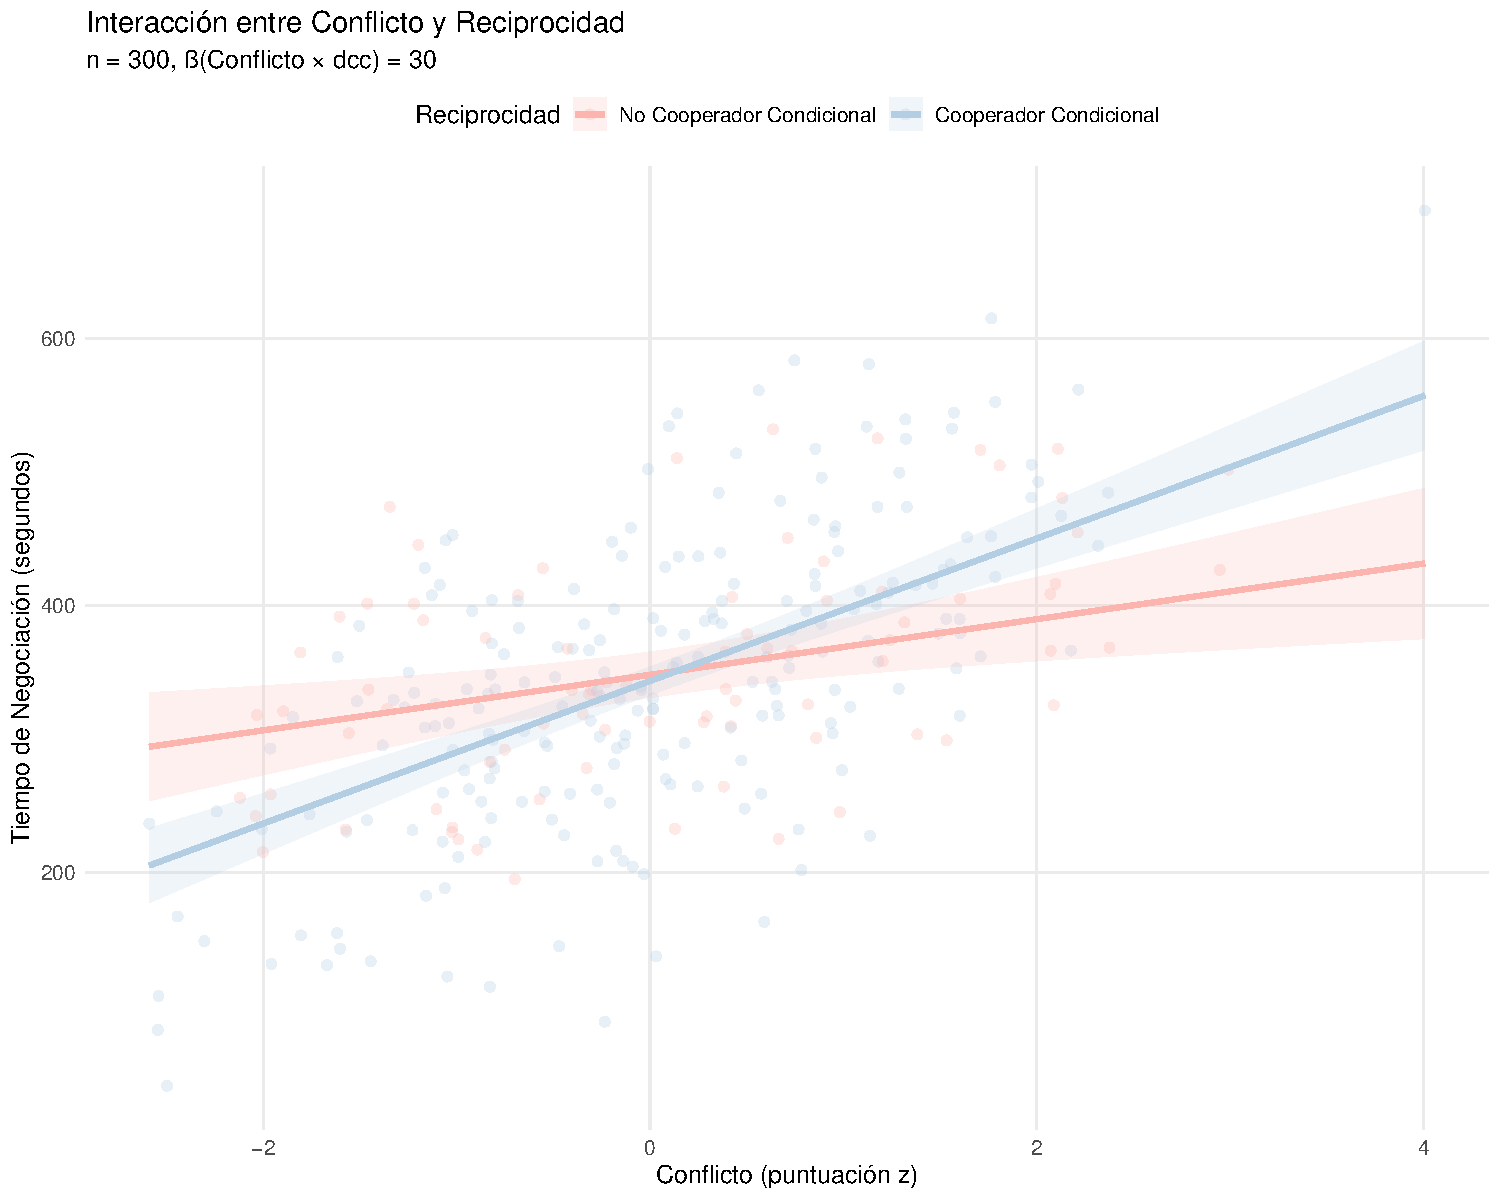
\includegraphics[keepaspectratio]{Prueba1_Amaru_Aguero_files/figure-pdf/fig-fig3-1.pdf}}

}

\caption{\label{fig-fig3}Interacción entre Conflicto y reciprocidad}

\end{figure}%

\newpage

\section{Pregunta 7.}\label{pregunta-7.}

Discutir principales resultados y plantear conclusiones del ejercicio y
los Modelos.

\newpage

\section{Repositorio GitHub y
Referencias.}\label{repositorio-github-y-referencias.}

Este
\href{https://github.com/AmaruSimonAgueroJimenez/Econometria-DCCS}{repositorio}
contiene el código fuente de este ejercicio, así como los datos
utilizados para la simulación y análisis. De igual manera se puede
acceder con el siguiente código QR.

\begin{center}
\pandocbounded{
\includegraphics[keepaspectratio]{Prueba1_Amaru_Aguero_files/figure-pdf/unnamed-chunk-11-1.pdf}}
\end{center}

El informe .pdf se encuentra en
\href{http://github.com/AmaruSimonAgueroJimenez/Econometria-DCCS/blob/main/docs/Prueba1_Amaru_Aguero.pdf}{esta
dirección}. De igual manera se puede acceder con el siguiente código QR.

\begin{center}
\pandocbounded{
\includegraphics[keepaspectratio]{Prueba1_Amaru_Aguero_files/figure-pdf/unnamed-chunk-12-1.pdf}}
\end{center}

\phantomsection\label{refs}
\begin{CSLReferences}{1}{0}
\bibitem[\citeproctext]{ref-gerpott2018how}
1. Gerpott, F. H., Balliet, D., Columbus, S., Molho, C., \& Vries, R. E.
de. (2018). How do people think about interdependence? A
multidimensional model of subjective outcome interdependence.
\emph{Journal of Personality and Social Psychology}, \emph{115}(4),
716-742. \url{https://doi.org/10.1037/pspp0000166}

\bibitem[\citeproctext]{ref-fischbacher2012behavioral}
2. Fischbacher, U., Gächter, S., \& Quercia, S. (2012). The behavioral
validity of the strategy method in public good experiments.
\emph{Journal of Economic Psychology}, \emph{33}(4), 897-913.
\url{https://doi.org/10.1016/j.joep.2012.04.002}

\bibitem[\citeproctext]{ref-murphy2011measuring}
3. Murphy, R. O., Ackermann, K. A., \& Handgraaf, M. J. J. (2011).
Measuring social value orientation. \emph{Judgment and Decision Making},
\emph{6}(8), 771-781. \url{https://ssrn.com/abstract=1804189}

\end{CSLReferences}




\end{document}
